\section{Zweites Bonusfeature: Hilfestellung zur aktuellen Spielsituation}\label{sec:handy-help}
Das Spiel \textit{ Monster Odyssey} wird mit diesem Bonusfeature einsteigerfreundlicher, da der Nutzer beim ersten Einstieg in das Spiel eine kurze Einführung über das Spiel und die Tastenkombinationen mittels eines modernen, futuristischen Handys erhält. Darüber hinaus erhält der Nutzer Unterstützung in bestimmten Situationen. Beispielsweise erscheinen einige Benachrichtigungen beziehunsgweise Hilfestellungen, nachdem der Nutzer das Starter-Monster erhalten oder der Nutzer einen Kampf verloren hat und seine Monster keine Lebenspunkte mehr haben.
\subsection{Mockups}\label{subsec:mockups-handy-help}
Wenn der Nutzer zum ersten Mal in das Spiel einsteigt, erscheint eine Glocke oben rechts, wie in Abbildung~\ref{fig: Benachrichtigung beim Erhalt einer Nachricht} neben dem futuristischen Handy zu sehen ist.
Die Glocke bedeutet, dass es mindestens eine ungelesene Nachricht von dem Alien Meruem gibt.
Der Nutzer kann diese Nachrichten lesen, indem er in der oberen rechten Ecke auf das Handy, wie in der Abbildung~\ref{fig: Benachrichtigung beim Erhalt einer Nachricht} drückt. 
Meruem hat bereits bei der Willkommensszene dem Nutzer geholfen und somit ist er auch im Spiel der Begleiter des Nutzers.
Zuerst begrüßt Meruem den Nutzer und heißt ihn in das Spiel willkommen.
Danach hinterlässt Meruem als Hilfestellung Nachrichten bei dem Nutzer. Meruem teilt dem Nutzer zum Beispiel mit, dass er seinen Trainer bewegen kann und welche Interaktionstaste gewählt ist. 
Darüber hinaus verweist er den Nutzer auf den NPC-Trainer Prof. Albert, bei dem Starter-Monster erworben werden können. Eine Beispieldarstellung dieser Nachrichten ist in der Abbildung~\ref{fig: Vierte Nachricht} zu finden.
\begin{figure}[H]
    \center
    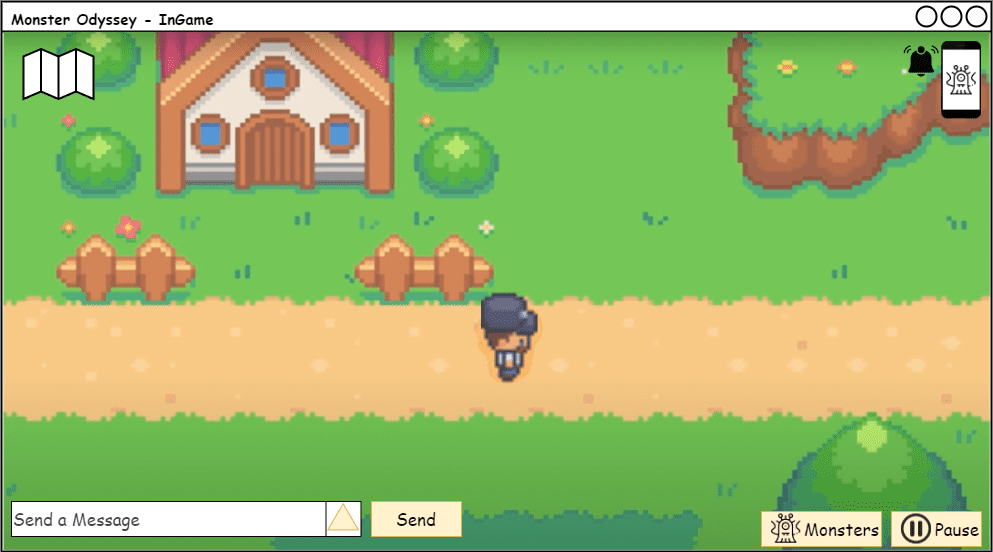
\includegraphics[scale=\scale]{images/mockups/Bonusfeatures/Helpsituation/PlayerAndPlayerIngame.png}
    \caption{Mockup: Benachrichtigungssymbol beim Erhalt einer Nachricht}
    \label{fig: Benachrichtigung beim Erhalt einer Nachricht}
\end{figure}
\begin{figure}[H]
        \center
        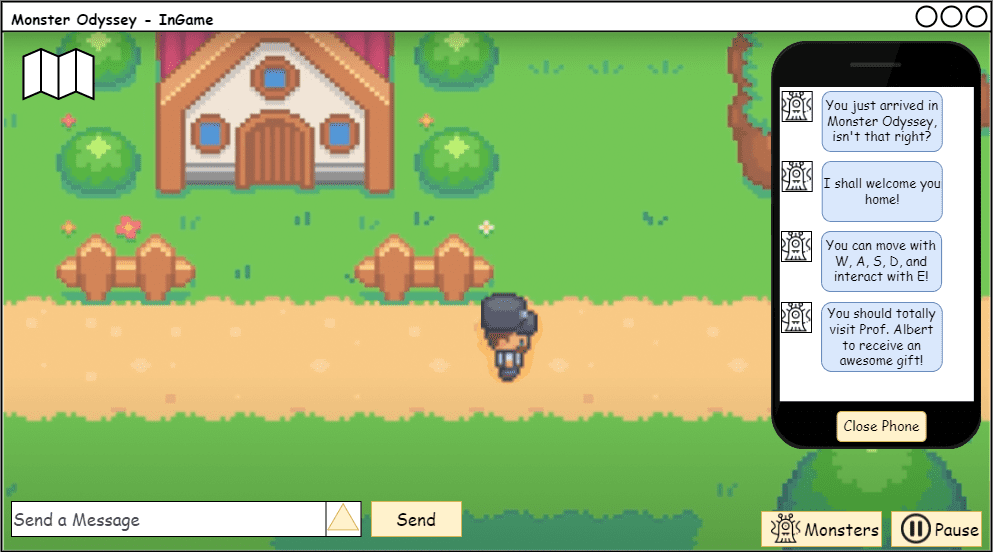
\includegraphics[scale=\scale]{images/mockups/Bonusfeatures/Helpsituation/PlayerAndPlayerIngameFourthNotification.png}
        \caption{Hilfestellung beim Einstieg}
        \label{fig: Vierte Nachricht}
\end{figure}
Der Nutzer erhält von Meruem Nachrichten nach bestimmten Ereignissen.
Beispielsweise bekommt der Nutzer nach dem Erhalt von dem Starter-Monster zwei Nachrichten von Meruem wie in der Abbildung~\ref{fig: Sechste Nachricht}, in denen der Nutzer aufgerufen wird, seine Fähigkeiten unter Beweis zu stellen, mit anderen Trainern zu interagieren und gegen diese zu kämpfen.
Weiterhin erhält der Nutzer Hilfestellung von Meruem nach dem Verlust eines Kampfs oder bei niedrigen Lebenspunkten der eigenen Monster wie in der Abbildung~\ref{fig: Achte Nachricht}, indem Meruem den Nutzer auf die Krankenschwester im 'Moncenter' verweist, um die Monster zu heilen.
\begin{figure}[H]
        \center
        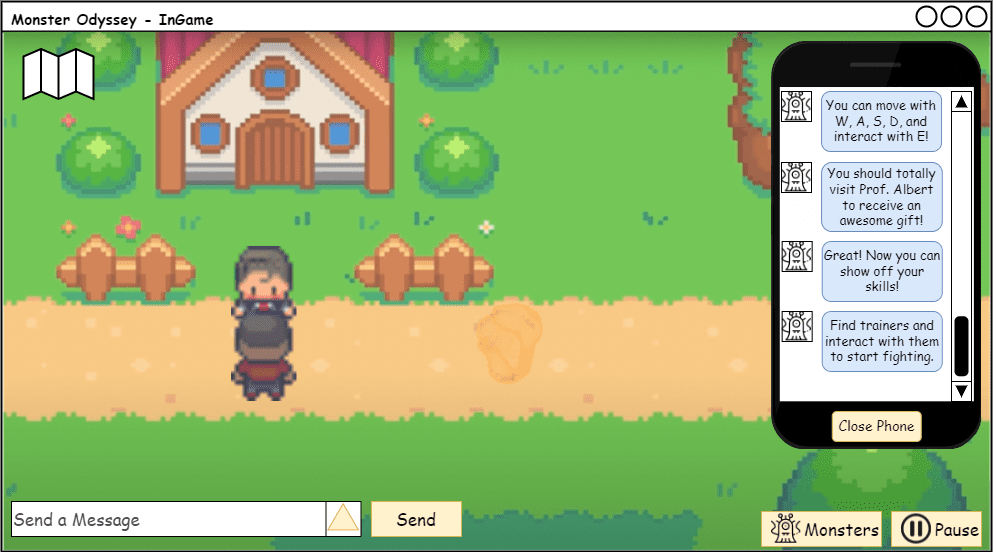
\includegraphics[scale=\scale]{images/mockups/Bonusfeatures/Helpsituation/PlayerAndPlayerIngameSixthNotification.png}
        \caption{Hilfestellung beim Erhalt eines Starter-Monsters}
        \label{fig: Sechste Nachricht}
\end{figure}
\begin{figure}[H]
        \center
        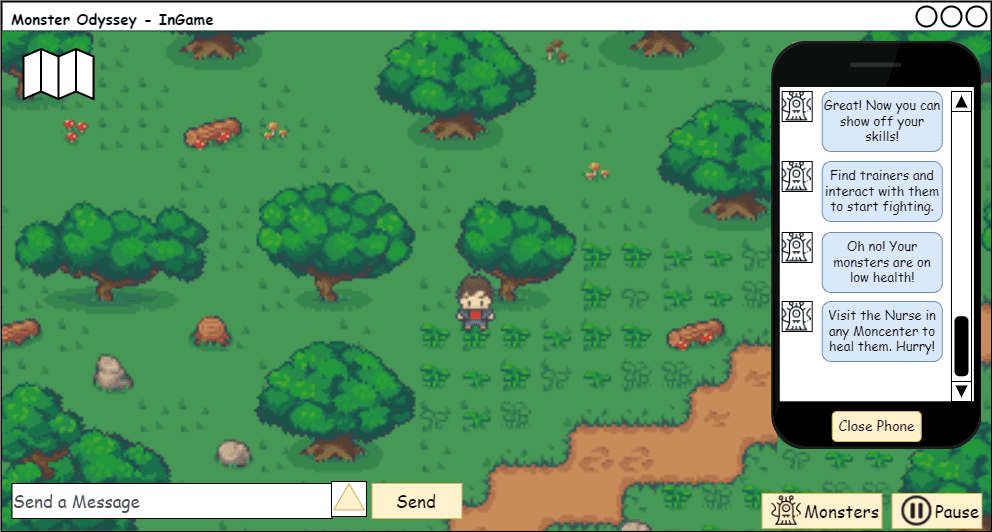
\includegraphics[scale=\scale]{images/mockups/Bonusfeatures/Helpsituation/PlayerAndPlayerIngameEigthNotification.png}
        \caption{Hilfestellung bei niedrigen Lebenspunkten der Monster}
        \label{fig: Achte Nachricht}
\end{figure}
\subsection{Vergleich zwischen Mockups und Implementierung}\label{subsec:vergleich-zwischen-mockups-und-implementierung-handy-help}
In der Abbildung~\ref{fig: Vergleich: Einstiegshilfe} bestehen zwischen dem Mockup und der Implementierung zwei Unterschiede. Zunächst enthält der Knopf für das Schließen in der Abbildung~\ref{fig: Implementierung: Einstiegshilfe} nur den Text 'Close', da bei der Übersetzung in die angebotenen Sprachen der Text viel Platz in Anspruch genommen hätte. Außerdem hat das Bild für Meruem keinen Behälter, was allerdings keinen Einfluss auf die Mechanik oder das Spielerlebnis hat. Dieser wurde wegen zunehmender Komplexität des Handys und der Nachrichten weggelassen.
\begin{figure}[H]
    \centering
    \begin{subfigure}[b]{0.4\textwidth}
        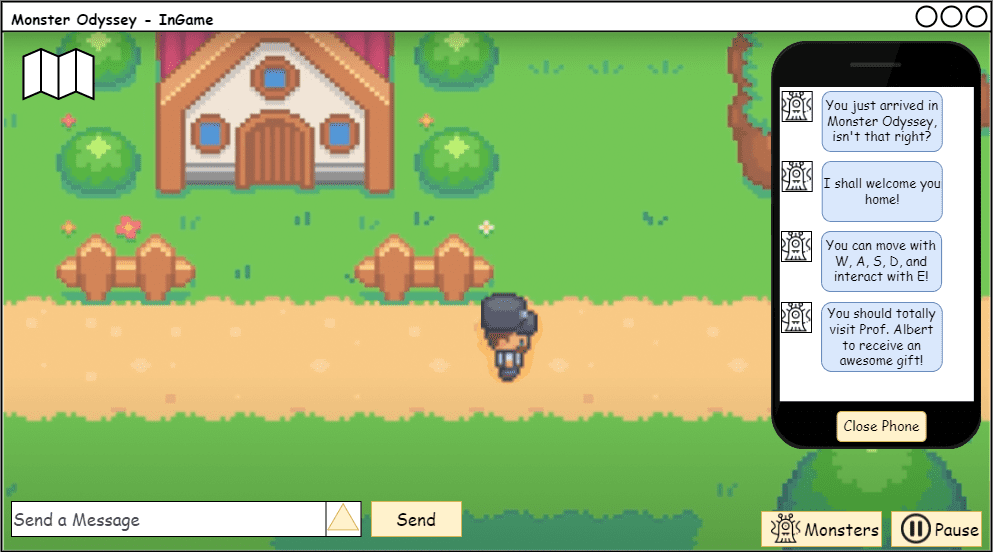
\includegraphics[width=\textwidth]{images/mockups/Bonusfeatures/Helpsituation/PlayerAndPlayerIngameFourthNotification.png}
        \caption{Mockup: Einstiegshilfe}
        \label{fig: Mockup: Einstiegshilfe}
    \end{subfigure}
    \hfill
    \begin{subfigure}[b]{0.4\textwidth}
        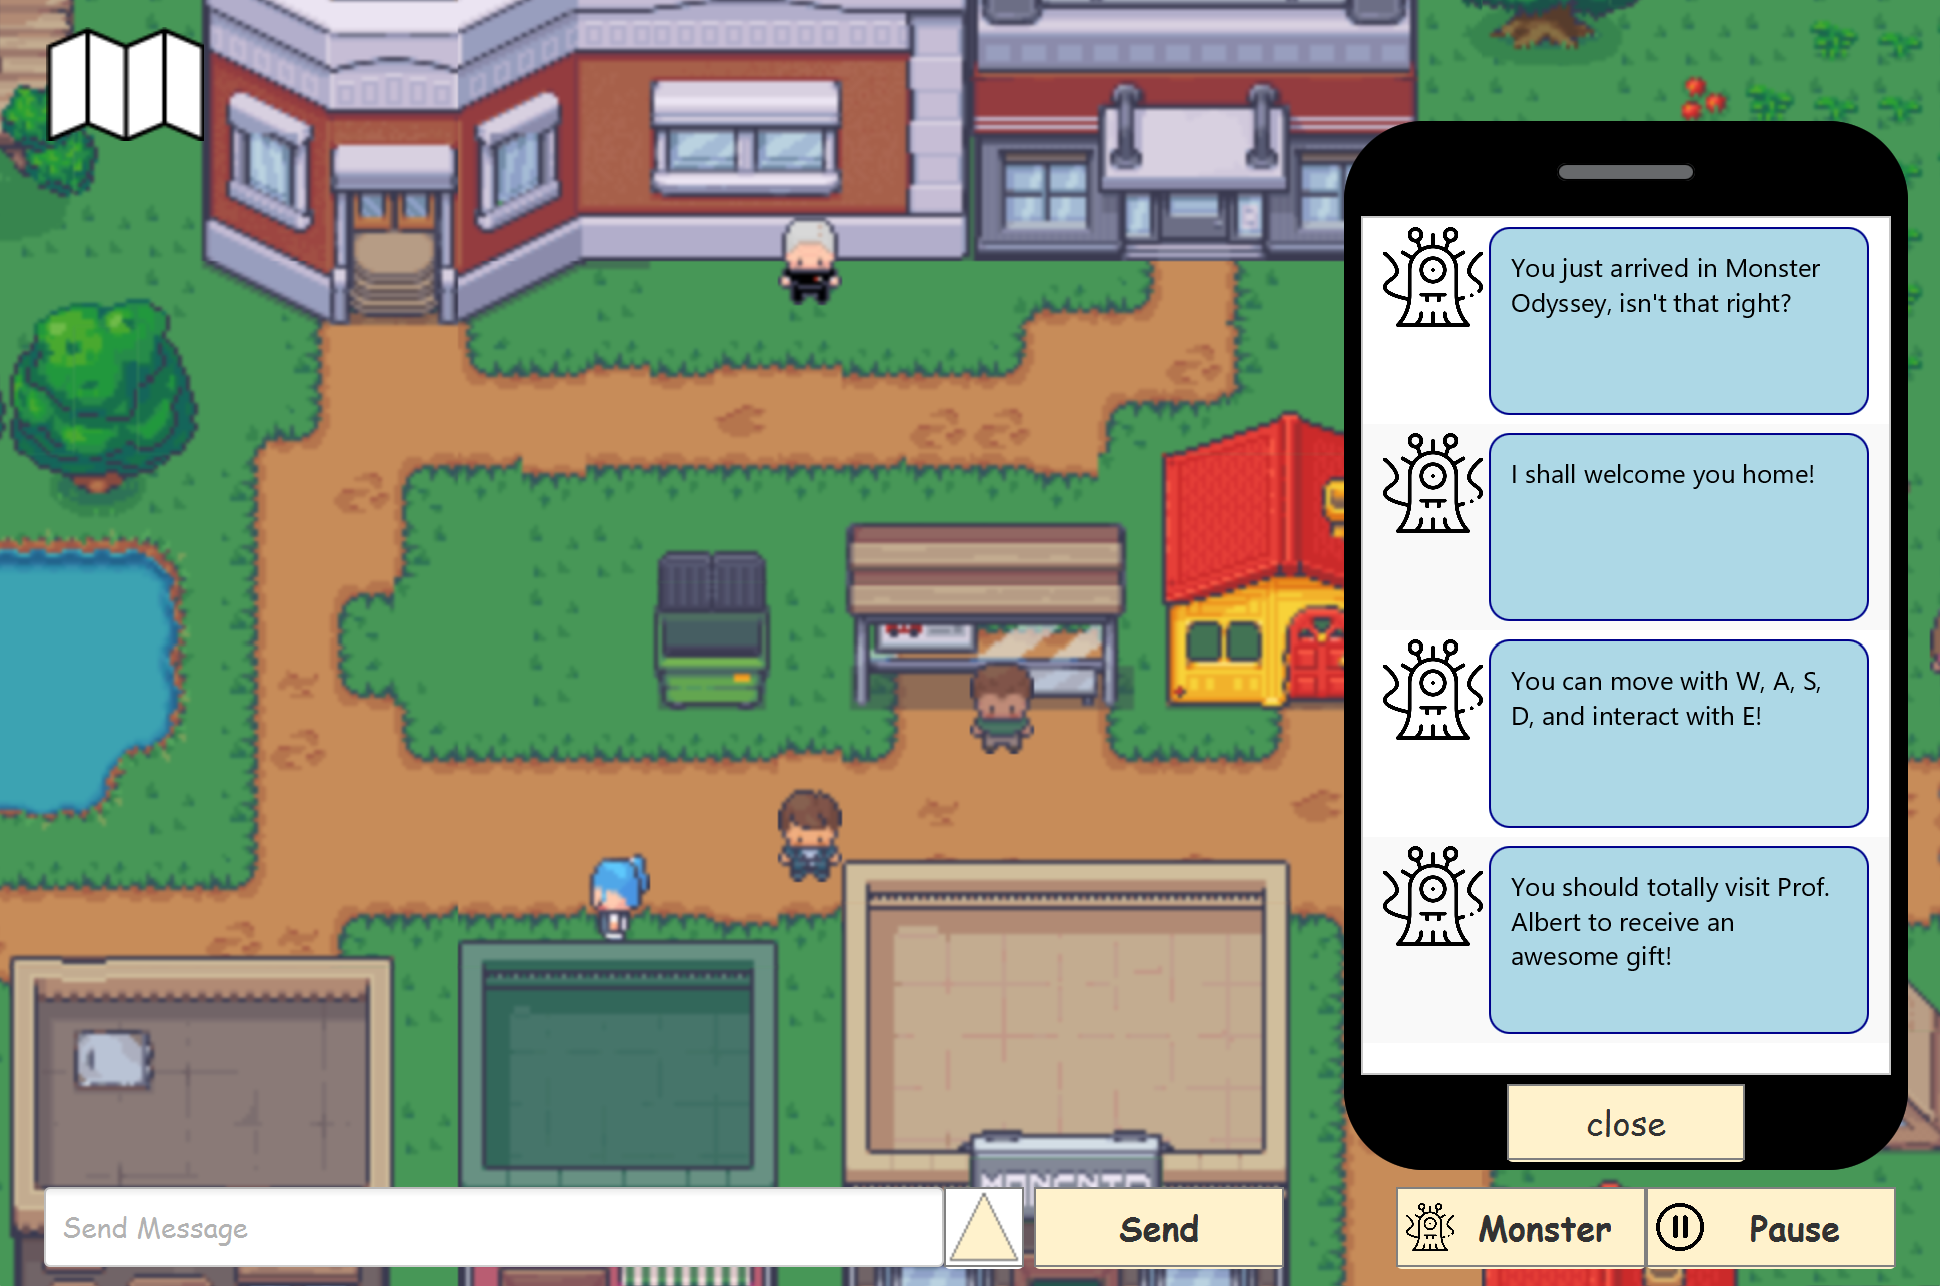
\includegraphics[width=\textwidth]{images/implementation/Bonusfeatures/Helpsituation/FirstMessagesImp.png}
        \caption{Implementierung: Einstiegshilfe}
        \label{fig: Implementierung: Einstiegshilfe}
    \end{subfigure}
    \caption{Vergleich: Einstiegshilfe}
    \label{fig: Vergleich: Einstiegshilfe}
\end{figure}
Überdies besteht noch ein wesentlicher Unterschied beim Vergleich in der Abbildung~\ref{fig: Vergleich: Nach Erhalt des Starter-Monsters} bezüglich der Hilfestellung nach Auftreten eines Ereignisses. Hierfür wurden die vorherigen Nachrichten in der Implementierung entfernt, um das Handy nicht dauherhaft zu überladen. Das erleichtert das Lesen der Nachrichten auf dem Handy.
\begin{figure}[H]
    \centering
    \begin{subfigure}[b]{0.4\textwidth}
        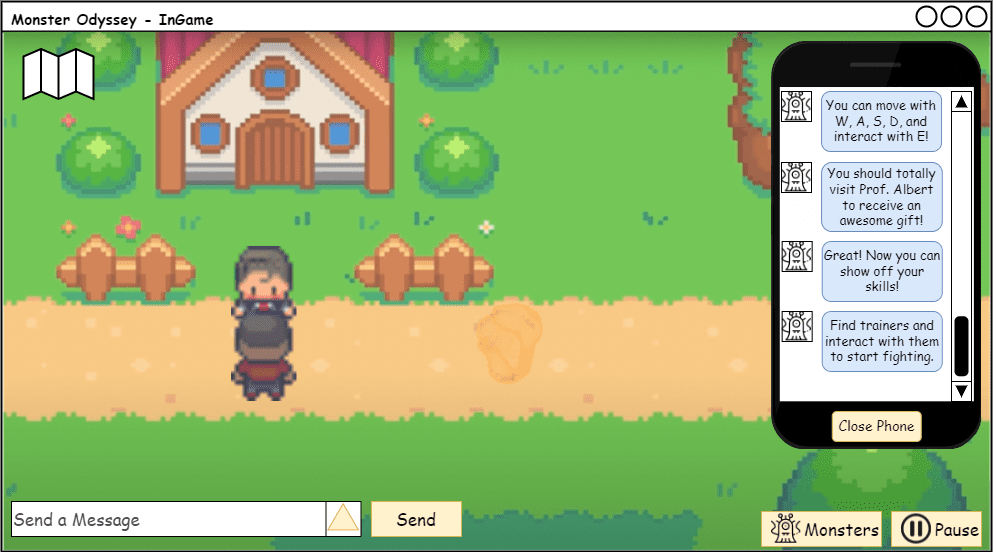
\includegraphics[width=\textwidth]{images/mockups/Bonusfeatures/Helpsituation/PlayerAndPlayerIngameSixthNotification.png}
        \caption{Mockup: Nach Erhalt des Starter-Monsters}
        \label{fig: Mockup: Nach Erhalt des Starter-Monsters}
    \end{subfigure}
    \hfill
    \begin{subfigure}[b]{0.4\textwidth}
        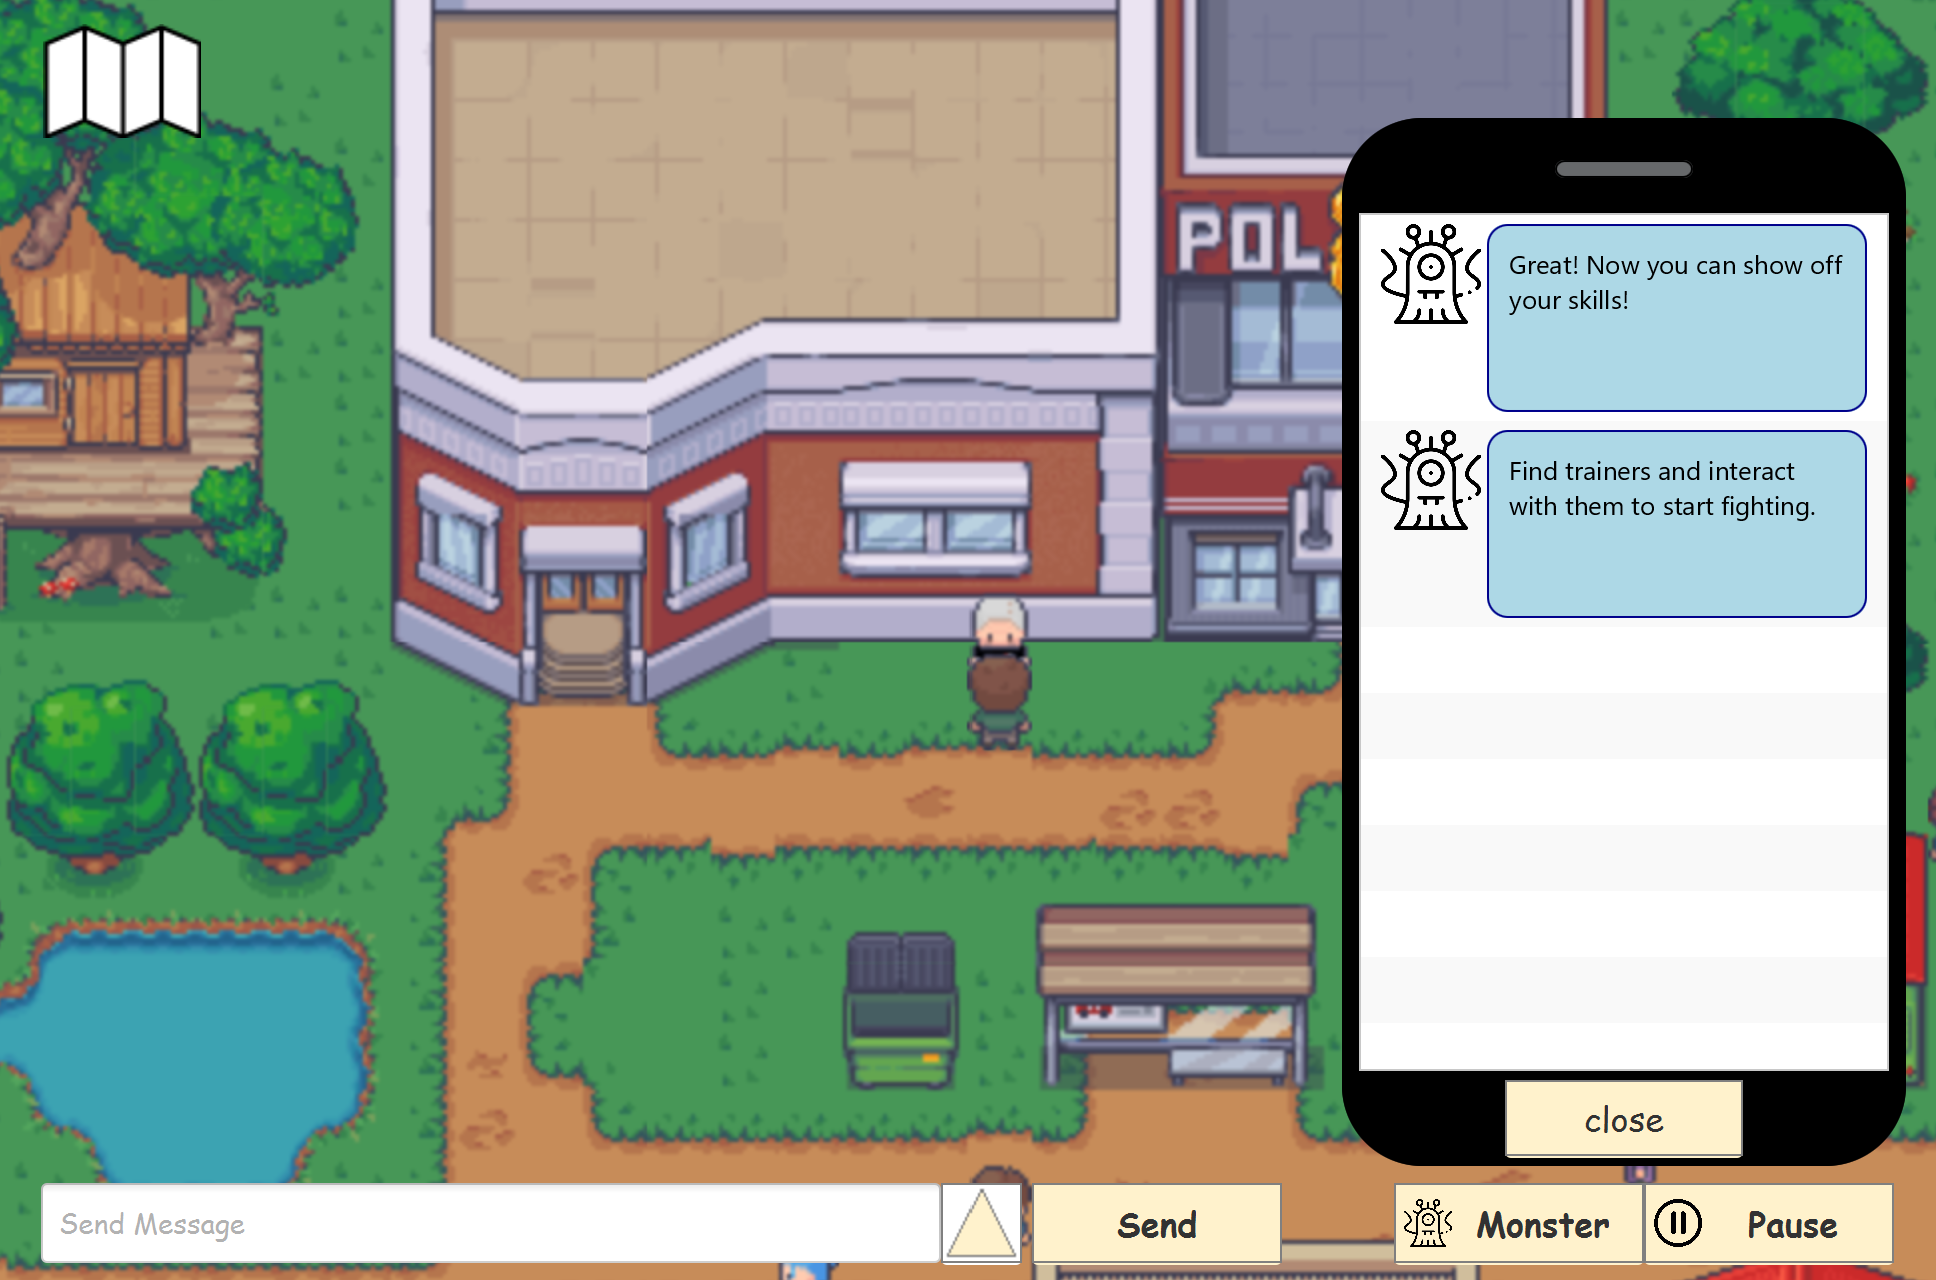
\includegraphics[width=\textwidth]{images/implementation/Bonusfeatures/Helpsituation/StarterMonsterMessagesImp.png}
        \caption{Implementierung: Nach Erhalt des Starter-Monsters}
        \label{fig: Implementierung: Nach Erhalt des Starter-Monsters}
    \end{subfigure}
    \caption{Vergleich: Nach Erhalt des Starter-Monsters}
    \label{fig: Vergleich: Nach Erhalt des Starter-Monsters}
\end{figure}